% Copyright (C)  2011  Dennis Ideler (dennisideler.com)
%    Permission is granted to copy, distribute and/or modify this document
%    under the terms of the GNU Free Documentation License, Version 1.3
%    or any later version published by the Free Software Foundation;
%    with no Invariant Sections, no Front-Cover Texts, and no Back-Cover Texts.
%    A copy of the license is included in the section entitled "GNU
%    Free Documentation License" at http://www.gnu.org/copyleft/fdl.html
%
% Instructions: print double sided, 4 pages per sheet

\documentclass[8pt,letterpaper,twocolumn]{article}
\usepackage{fullpage}
\usepackage{setspace}
\usepackage{algorithm}
\usepackage{algorithmic}
\usepackage[latin1]{inputenc}
\usepackage{amsmath}
\usepackage{amsfonts}
\usepackage{amssymb}
\usepackage{graphicx}
\usepackage{upgreek} % for /Upphi, /Upgamma, etc.

\addtolength{\textwidth}{2cm}
\addtolength{\hoffset}{-1cm}
\addtolength{\textheight}{2cm}
\addtolength{\voffset}{-2cm}

\begin{document} % Everything from A1 + A2 + notes, up to, but not including Grammar.
\section*{Theory of Computation Cheat Sheet}
\underline{\textbf{Induction}}\\ % because sections use too much space!
\\
Proof by induction has two steps: proving the base case and the inductive step.
These two parts should convince us that $S(n)$ is true for every integer $n$
that is equal to or greater than the basis.\\
\\
\textbf{E.g.} Prove $S(n) = n! > 2^n$ for $n \geq 4$\\
\\
\textbf{Step 1: Basis}\\ % Prove base case
$S(4) = 4! > 2^4 = 24 > 16$.\\
\\
\textbf{Step 2: Induction}\\
Inductive hypothesis: assume true for $k \geq 4$.\\
If $S(k) = k! > 2^k$ then $S(k+1) = (k+1)! > 2^{k+1}$.\\
Rewrite $S(k+1)$ so it can make use of $S(k)$.\\
$S(k+1) = (k+1)\,k! > 2 \cdot 2^k$\\
$S(n)$ tells us that $k! > 2^k$.
If we remove that assumed truth from the above statement, we only need to show $k+1 > 2$.
Since $n \geq 4$, we get $4 + 1 > 2$ which holds.\\
\\
\underline{\textbf{Technique of Diagonalization}}\\
\\
Diagonalization is used to \underline{show that a set is uncountable}.
An uncountable set is an infinite set that contains too many elements to be countable
(i.e. it is \underline{not enumerable}).
The uncountability of a set is closely related to its cardinal number:
a set is uncountable if its cardinal number is larger than that of the set of all natural numbers.
The set of natural numbers (and any other countably infinite set) has cardinality aleph-null
($\aleph_0$).\\
\\
1: Assume set is countable, enumerate all subsets\\
2: Create new subset using elements from existing subsets\\
3: Show new subset is in set but not in enumeration\\
\\
\underline{E.g.} A function $f : N \rightarrow N$ is monotone-increasing if
$f(i) < f(i+1) \: \forall \: i \in N$.
Prove, using diagonalization, that the set of monotone-increasing functions is uncountable.\\
\\
1) Assume set of all monotone-increasing functions is countable
\begin{tabular}{c|c c c c c}
& 1 & 2 & 3 & $\cdots$ & $i$ \\
\hline
$f_1$ & \textbf{1} & 2 & 3 & $\cdots$\\
$f_2$ & 2 & \textbf{4} & 6 & $\cdots$\\
$f_3$ & 3 & 5 & \textbf{7} & $\cdots$\\
$\vdots$\\
$f_i$\\
\end{tabular}
\\
2) Create a new monotone-increasing function $f(i) = f(i-1) + f_i(i),\: f \neq f_i \: \forall \: i$.\\
$f(1) = 0 + f_1(1) = 0 + 1 = 1\\
f(2) = 1 + f_2(2) = 1 + 4 = 5\\
f(3) = 5 + f_3(3) = 5 + 7 = 12\\
\vdots$\\
\\
3) $f(i) \in N$ but not in enumeration (differs in some column with every row).
$\therefore$ the set of monotone-increasing functions is uncountably infinite.\\
\\
\underline{E.g.} Prove, using diagonalization, that the power set of natural numbers ($2^N$) is uncountable.\\
\\
1) Assume $2^N$ is countable. Enumerate all subsets (in binary representation)
\begin{tabular}{c|c c c c c}
& 1 & 2 & 3 & $\cdots$ & $N$ \\
\hline
$S_1$ & \textbf{0} & 0 & 0 & $\cdots$\\
$S_2$ & 1 & \textbf{1} & 1 & $\cdots$\\
$S_3$ & 1 & 0 & \textbf{1} & $\cdots$\\
$\vdots$\\
$S_i$\\
\end{tabular}\\
2) Create a new subset $S(i) = 1-S_i(i), \: S \neq S_i \: \forall \: i$.\\
$S(1) = 1 - S_1(1) = 1 - 0 = 1\\
S(2) = 1 - S_2(2) = 1 - 1 = 0\\
S(3) = 1 - S_3(3) = 1 - 1 = 0\\
\vdots$\\
\\
3) $S(i) \in 2^N$ (because the power set contains all subsets of set $N$) but not in enumeration.
$\therefore$ the power set of all natural numbers is uncountably infinite.\\
\\
\underline{\textbf{Set Theory}}\\
\\
Sets are (1) well defined, (2) have no ordering of elements, and (3) contain no duplicates -- but
multi-sets do.\\
\underline{Definitions}
\begin{tabular}{|c|c|}
\hline 
$A :$ set & $A$ is a set \\ 
\hline 
$x \in A$ & $x$ is an element/member of $A$ \\ 
\hline
$\emptyset, \{\}$ & empty set\\
\hline 
$\emptyset \subseteq A$ & empty set is a subset \\
\hline
$A \subseteq A$ & set is a subset of itself \\
\hline
$A \subseteq B$ & $A$ is a subset of $B$ if $a \in A, a \in B$ \\
$A \subset B$ & proper subset if $a \in A, a \in B, A \neq B$ \\
\hline
$2^A$ & power set (all subsets of set $A$) \\
\hline
$\left|A\right|$ & cardinality of $A$ (number of elements) \\
\hline
$2^{|A|}$ & number of subsets of $A$\\
\hline
\end{tabular}
\underline{Operations}
\begin{tabular}{|c|c|}
\hline
Union & $A \cup B = \{x \mid x \in A$ or $x \in B \}$ \\
& e.g. $\{1,2\} \cup \{2,3\} = \{1,2,3\}$ \\
\hline
Intersection & $A \cap B = \{x \mid x \in A$ and $x \in B\}$ \\
& e.g. $\{1,2\} \cap \{2,3\} = \{2\}$ \\
\hline
Set Difference & $A - B = \{x \mid, x \in A, x \notin B\}$ \\
& e.g. $\{1,2\} \setminus \{2,3\} = \{1\}$ \\
\hline
Cartesian Product & $A \times B = \{(a,b) \mid a \in A, b \in B\}$ \\
\hline
Complement & everything not in the set \\
\hline
\end{tabular}
\underline{Properties}
\begin{tabular}{|c|c|}
\hline
Commutative & $A \cup B = B \cup A$ \\
& $A \cap B = B \cap A$ \\
\hline
Associative & $A \cup (B \cup C) = (A \cup B) \cup C$ \\
& $A \cap (B \cap C) = (A \cap B) \cap C$ \\
\hline
Distribution & $A \cap (B \cup C) = (A \cap B) \cup (A \cap C)$ \\
& $A \cup (B \cap C) = (A \cup B) \cap (A \cup C)$ \\
\hline
\end{tabular}
\\
\underline{E.g.} Is the set of all functions $f:\{0,1\} \rightarrow N$ countable?\\
\\
This function has two cases: $f_i(0) \rightarrow N$ and $f_i(1) \rightarrow N$.\\
$|N| = \aleph_0$ which means the set of $N$ is countable.
$f:\{0,1\} \rightarrow N$ is equivalent to
$f:\{0\} \rightarrow N \, \bigcup \, f:\{1\} \rightarrow N$.\\
The union of two countable sets results in a countable set, $N \bigcup N = N$
thus $f:\{0,1\} \rightarrow N$ is countably infinite.\\
\\
\underline{\textbf{One-to-one and Onto Functions}}\\
$\bullet \: A$ onto $B \Rightarrow$ every element in $B$ is mapped\\
$\bullet \: A$ 1-1 $B \Rightarrow$ every element in $A$ has a unique mapping\\
$\bullet$ 1-1 correspondence $\Rightarrow$ bijective (1-1 \emph{and} onto).
\emph{i.e.} No two values map to the same value.
Every element in the codomain is mapped. $|A| = |B|$, same cardinality.\\
$\bullet$ Identity function $\Rightarrow$ input parameter is the same as the output value.\\
$\bullet$ A function has a single outcome for each parameter\\
\\
\underline{E.g.} functions $f:N \rightarrow N$ where $N = \{1,2,3,\dots\}$
\begin{enumerate}
  \item $f$ is 1-1 but not onto:\\
  $f(x) = x + 1$\\
  $f(1) = 2$\\
  $f(2) = 3$\\
  $f(3) = 4$\\
  $\vdots$
  
  \item $f$ is onto but not 1-1:\\
  $f(x) = \lceil \frac{x}{2} \rceil$\\
  $f(1) = 1$\\
  $f(2) = 1$\\
  $f(3) = 2$\\
  $f(4) = 2$\\
  $f(5) = 3$\\
  $f(6) = 3$\\
  $\vdots$
  
  \item $f$ is a 1-1 correspondence and not an identity function:\\
  $f(x) = x - (x + 2 \: mod \: 3) + (x \: mod \: 3)$\\
  $f(1) = 2$\\
  $f(2) = 3$\\
  $f(3) = 1$\\
  $f(4) = 5$\\
  $f(5) = 6$\\
  $f(6) = 4$\\
  $\vdots$\\
  Conditional functions would also work.
\end{enumerate}
\underline{\textbf{Countability}}\\
Set $A$ is countable if $\exists$ a 1-1 correspondence between $A$ and $N$.
i.e. Can systematically enumerate all elements in $A$ eventually, labeling each with
a unique natural number. You might have to find a creative pattern to list them 1-by-1.\\
\\
\underline{E.g.} Set of $\pm$ rational numbers is countable if you enumerate as
$x_1, \, -x_1, \, x_2, \, -x_2, \, \cdots$\\
\\
\underline{E.g.} $N \times N \times N$ is countable. 3-tuple $(i,j,k)$.
If $a=1$, there are $a^3$ tuples (finite) such that
$1 \leq i \leq a, \: 1 \leq j \leq a, \: 1 \leq k \leq a$.
Finite if $a=2,3,\cdots$\\
\\
\underline{E.g.} $\left| (0,1) \right| = \left| 2^N \right| = \aleph_1 = $ uncountable.
($\aleph_0$ is countable)\\
\\
\underline{E.g.} Set of binary functions $f:N \rightarrow \{0,1\}$ is uncountable.\\
\\
\underline{\textbf{Languages}}\\
%TODO: A1, A2, lecture notes, online notes, old tests
$\bullet$ An alphabet $\Sigma$ is a finite set of symbols, e.g. $\Sigma = \{0,1\}$\\
$\bullet$ A language over alphabet $\Sigma$ is a set of strings,
each having its characters drawn from $\Sigma$\\
$\bullet$ Length of a string $s,\, |s|$, is the \# of symbols in string $s$\\
$\bullet$ Empty string $\epsilon$ has length 0\\
$\bullet$ Substrings of $abc = a,\, b,\, c,\, ab,\, bc,\, abc$\\
$\bullet$ Prefix is any \# of leading symbols, e.g. $\epsilon,\, a,\, ab,\, abc$\\
$\bullet$ Postfix is any \# of trailing symbols, e.g. $\epsilon, c,\, bc,\, abc$\\
$\bullet$ Reversal is the string in reverse, e.g. $s = abc, \: s^R = cba$\\
Special languages:
\begin{enumerate}
\item $\emptyset$ is the empty language
\item $\{\epsilon\}$ language that contains empty string
\item $\Sigma^*$ (Kleene Closure) contains all strings over $\Sigma$
\item $\Sigma^+$ (Positive Closure) contains all strings over $\Sigma$ except the empty string
\end{enumerate}
\underline{Operations}
\begin{tabular}{|c|c|}
\hline 
Concatenation & $\{a\} \cdot \{b\} = \{a\}\{b\} = \{ab\}$ \\ 
\hline 
Union & $\{a\}\, \cup$ or $+$ or $\mid \{b\} = \{a,b\}$ \\ 
\hline
Kleene Closure & $\{a\}^* = \{\epsilon,\, a,\, aa,\, aaa,\, \cdots\}$ \\ 
\hline
Positive Closure & $\{a\}^+ = \{a,\, aa,\, aaa,\, \cdots\}$ \\
\hline
\end{tabular}
\\
\underline{E.g.} First 5 strings of language $L = \{x \in \{a,b,c\}^* : x$
contains at least one $a$ and at least one $b\}$ in lexicographical order.
$\Rightarrow ab,\, ba,\, aab,\, aba,\, abb$\\
\\
\underline{E.g.} Let $X = \{aa, bb\}$ and $Y = \{\epsilon, b, ab\}$.
\begin{enumerate}
  \item List the strings in the set $XY$.\\
  $XY = X \cdot Y = \{aa, bb\}\{\epsilon, b, ab\}$\\
  $ = \{aa,\, aa b,\, aa ab,\, bb,\, bb b,\, bb ab\}$

  \item List the strings of the set $Y^*$ of length three or less.\\
  $Y^* = \{\epsilon, b, ab\}^*$ of length 3 or less\\
  $= \{\epsilon,\, b,\, b b,\, b b b,\, ab,\, b ab,\, ab b\}$

  \item How many strings of length 6 are there in $X^*$?\\
  $X^* = \{aa,bb\}^*$ of exactly length 6\\
  Each symbol has length 2, so there have to be 3 symbols in each string. $2^3 = 8$ strings.
  \begin{enumerate}
  	\item $000 \rightarrow aa aa aa$
 	\item $001 \rightarrow aa aa bb$
  	\item $010 \rightarrow aa bb aa$
  	\item $011 \rightarrow aa bb bb$
  	\item $100 \rightarrow bb aa aa$
  	\item $101 \rightarrow bb aa bb$
  	\item $110 \rightarrow bb bb aa$
  	\item $111 \rightarrow bb bb bb$
  \end{enumerate}
\end{enumerate}

\underline{E.g.} Let $L_1 = \{aaa\}^*$, $L_2 = \{a,b\}\{a,b\}\{a,b\}\{a,b\}$, and $L_3 = L_2^*$.
Describe the strings that are in the languages.
\begin{enumerate}
  \item $L_2 =$ strings of length 4 that are any combination of $a$'s and $b$'s.
  \item $L_3 =$ closure of $L_2$, 0 or more occurrences of $L_2$.
  i.e. empty string and strings that are a multiple of 4 with any combination of $a$'s and $b$'s.
  E.g. $\epsilon$, $aaab$, $bbbbaaaa$, etc.
  \item $L1 \bigcap L_3 =$ intersection of $L_1$ and $L_3$, which are strings of symbol $aaa$
  that are multiples of 12. $L1 \bigcap L_3 = \{aaa\,aaa\,aaa\,aaa\}^*$
\end{enumerate}
\textbf{To show a language is regular:} show one option exists
\begin{enumerate}
\item regular expression
\item DFA
\item NFA
\item NFA w/ $\epsilon$-moves
\end{enumerate}
If $L$ is finite, it is regular.\\
\\
\textbf{To show a language is irregular:}
\begin{enumerate}
\item Pumping lemma
\item Show DFA that would require infinite states
\item Use closure properties that relate to other nonregular languages
\end{enumerate}
\textbf{Closure Properties} of regular languages:\\
Regular languages are closed under certain operations
(i.e. if $L_1, L_2$ are regular, then so is resulting language).
\begin{tabular}{|c|c|}
\hline 
Union & $L_1 \cup L_2 = r + s$ \\ 
Concatenation & $L_1 \cdot L_2 = rs$ \\ 
Closure & $L_1^* = r^*$, $L_2^+ = s^+$ \\
Complement & $\bar{L} = \Sigma^* - L$, ($L$ regular, so is $\bar{L}$)\\
Intersection & $L_1 \cap L_2 = \overline{\overline{L_1} \cup \overline{L_2}}$ \\
Set difference & $L_1 - L_2 = L_1 \cap \overline{L_2}$ \\
\hline 
\end{tabular} \\
\\
\underline{E.g.} For any fixed $n$, is $\bigcup_{i=1}^n L_i$ regular, where each $L_i$ is regular?\\
\\
True. $L_i$ is regular so has regex $r_i$.
Finite languages, so $\bigcup_{i=1}^n L_i$ has regex $r_1+r_2+\cdots+r_n$.\\
\\
\underline{E.g.}
Give examples of languages $L_1$ and $L_2$ over alphabet $\{a,b\}$ that satisfy\footnote{Hints:
Known regular languages: $\Sigma^*, \epsilon, a^*, a^* b^*,$ etc.
Known nonregular languages: $a^n b^n$ or languages with similar dependencies.}:
  \begin{enumerate}
  \item $L_1$ is regular, $L_2$ is nonregular, and $L_1 \bigcup L_2$ is regular.\\
  $L_1 = \{a,b\}^*,\, L_2 = \{a^n b^n | n \geq 0\} \rightarrow L_1 \bigcup L_2 = a^* b^*$\\
  $L_1 = a^*,\: L_2 = \{a^i \mid i$ is prime$\} \rightarrow L_1 \bigcup L_2 = L_1$
  
  \item $L_1$ is regular, $L_2$ is nonregular, and $L_1 \bigcup L_2$ is nonregular.\\
  $L_1 = \{a^*\},\, L_2 = \{a^n b^n | n \geq 0\} \rightarrow L_1 \bigcup L_2$\\
  $L_1 = \{aa\},\: L_2 = \{a^i \mid i$ is prime$\} \rightarrow L_1 \bigcup L_2 = L_2$
  
  \item $L_1$ is regular, $L_2$ is nonregular, and $L_1 \bigcap L_2$ is regular.\\
  $L_1 = \{a^*\},\, L_2 = \{a^n b^n | n \geq 0\} \rightarrow L_1 \bigcap L_2 = a^*$\\
  $L_1 = \{aa\},\: L_2 = \{a^i \mid i$ is prime$\} \rightarrow L_1 \bigcap L_2 = L_1$
    
  \item $L_1$ is nonregular, $L_2$ is nonregular, and $L_1 \bigcup L_2$ is regular.\\
  $L_1 = \{a^i | i > 0,\, i$ is prime$\},\, L_2 = \{a^i | i > 0,\, i$ is not prime$\}$
  $\rightarrow L_1 \bigcup L_2 = a^+$\\
  $L_1 = \{a^i | i$ is prime$\},\, L_2 = \{a^i | i$ is not prime$\}$
  $\rightarrow L_1 \bigcup L_2 = a^*$
  \end{enumerate}
\underline{E.g.} Prove or disprove the following:
  \begin{enumerate}
  \item If $L^*$ is regular, then $L$ must be regular.\\
  \\
  False. For example, $L = \{a^{2^i} | i \geq 0\}$ is nonregular, but $L^*$ is.
  Or $L = \{a^i | i$ is prime$\}$
% Kleene closure ($L^* = \bigcup_{i=0}^\infty L_i$)
% Positive closure ($L^+ = \bigcup_{i=1}^\infty L_i = L \cdot L^*$).
  
  \item For any language $L$, $L^*$ must be regular
  (discuss both cases when $L$ is finite and infinite).\\
  \\
  If $L$ is finite, then $L$ must be regular (you can find a FSM or regex).
  And if $L$ is regular $\Rightarrow L^*$ is regular, because
  the Kleene star/closure is a regular operation under closure properties.
  Therefore, if $L$ is finite, $L^*$ must be regular.\\
  If $L$ is infinite, then it is nonregular because you would need an
  infinite number of states (you cannot find a FSM or regex).
  Therefore, if $L$ is infinite, $L^*$ can be regular or nonregular (i.e. it does not say anything).
  \end{enumerate}
\underline{\textbf{Regular Expressions}}\\
Regular expressions (regex) are sets in a nicer notation.
\begin{tabular}{|c|c|}
\hline
$01 = 0 \cdot 1 = \{01\}$ & Concatenation: 0 followed by 1\\
\hline 
$0+1 = \{0,1\}$ & Union: $0$ or $1$\\ 
\hline 
$0^* = \{0\}^*$ & Kleene closure: zero or more 0's\\ 
\hline
$0^+ = \{0\}^+$ & Positive closure: one or more 0's\\
\hline
$0? = \{\epsilon, 0\}$ & zero or one 0\\
\hline
$(0+1)^* = \{0,1\}^*$ &  all strings over $\{0,1\}$\\
\hline
$0^*10^*10^* = 0^* \cdot 1 \cdot 0^* \cdot 1 \cdot 0^*$ & strings containing exactly two 1's\\
\hline
$(0+1)^*11 = \{0,1\}^*\cdot \{1\} \cdot \{1\}$ & strings ending with 11\\
\hline
$0(1+10)^*+(1+10)^* $ & strings of 0's and 1's \\
$= \{0\} \cdot \{1,10\}^* \cup \{1,10\}^*$ & not containing substring 00\\
\hline
\end{tabular} 
\\
\\
\underline{\textbf{Deterministic Finite Automata (DFA)}}\\
DFA \& NFA are Finite State Machines (FSM).
They can only scan input once (i.e. new string requires new scan process) and have finite memory.
Unlike Turing machines.\\
\\
DFA's are 5-tuple: $M = (Q,\, \Sigma,\, \delta,\, q_0,\, F)$
\begin{tabular}{c c} 
$Q$ & finite set of states \\  
$\Sigma$ & finite alphabet \\
$q_0 \in Q$ & initial state \\
$F \subseteq Q$ & final states \\
$\delta$ & transition function $Q \times \Sigma \rightarrow Q$ \\
$\delta(q,a) = p$ &  where $q, P$ are states in $Q$ and $a$ is symbol in $\Sigma$\\
$L(M)$ & language accepted by machine $M$
\end{tabular}\\
\\
$\bullet$ Deterministic means you can predict the path it will take (unlike in NFA).\\
$\bullet$ Every DFA is an NFA.\\
$\bullet$ Easy method to make a DFA that cannot contain a certain substring,
is to make a DFA that has to accept that substring, and then complement the DFA
(non-final states become final and vice-versa: $\bar{F} = Q-F$).\\
\\
\underline{\textbf{Nondeterministic Finite Automata (NFA)}}\\
% http://en.wikipedia.org/wiki/Nondeterministic_finite-state_machine
NFA is a finite state machine where for each pair of state and input symbol there may be several
possible next states. This distinguishes it from DFA, where the next possible state is uniquely
determined. Although DFA and NFA have distinct definitions, they are equivalent, in that,
for any given NFA, one may construct an equivalent DFA, and vice-versa (powerset construction).
Both types of automata recognize only regular languages.\\
%\\
%An NFA, similar to a DFA, consumes a string of input symbols.
%For each input symbol it transitions to a new state until all input symbols have been consumed.
%Unlike a DFA, it is non-deterministic in that, for any input symbol,
%its next state may be any one of several possible states.
%Thus, in definition, the next state is an element of the power set of states.
%This element, itself a set, represents some subset of all possible states to be considered at once.\\
\\
An extension of NFA is NFA with $\epsilon$-moves, which allows a transformation to a new state
without consuming any input symbols (using $\epsilon$ as the symbol in the transition).\\
\\
Accepting an input is similar to that for DFA.
When the last input symbol is consumed, the NFA accepts if and only if there is some set of
transitions that will take it to an accepting state (it's allowed to reach a stuck state).
Equivalently, it rejects, if, no matter what transitions are applied,
it would not end in an accepting state.\\
\\
\underline{E.g.} Give the state diagram of an NFA (without $\epsilon$-moves)
that accepts the language $(ab)^* + a^*$ and convert it to a DFA using the standard algorithm.

\begin{figure}[h!]
  \centering
    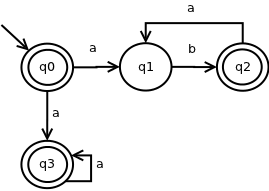
\includegraphics[scale=0.5]{nfa.png}
  \caption{NFA without $\epsilon$-moves for $(ab)^*+a^*$}
  \label{NFA}
\end{figure}
  
\begin{enumerate}
  \item $(ab)^* + a^* = (a \cdot b)^* \mid a^*$ = 0 or more $ab$'s or 0 or more $a$'s.\\
  \\
  For an NFA $M$, there exists a DFA $M'$ such that $L(M) = L(M')$.
  \begin{eqnarray*}
    M &=& (Q, \Sigma, \delta, q_0, F)\\
    Q &=& \{q_0,q_1,q_2,q_3\}\\
    \Sigma &=& \{a,b\}\\
    F &=& \{q_0,q_2,q_3\}\\
    \begin{tabular}{c|c|c|}
    $\delta$ & $a$ & $b$ \\ 
    \hline 
    $q_0$ & $\{q_1,q_3\}$ & $\emptyset$ \\
    \hline 
    $q_1$ & $\emptyset$ & $\{q_2\}$ \\ 
    \hline 
    $q_2$ & $\{q_1\}$ & $\emptyset$ \\ 
    \hline 
    $q_3$ & $\{q_3\}$ & $\emptyset$ \\ 
    \hline 
    \end{tabular} 
  \end{eqnarray*}
\\
  Each state in $M'$ corresponds to a subset of states from $M$.
  \begin{eqnarray*}
   M' &=& (Q', \Sigma, \delta', q_0', F')\\
   Q' &=& 2^Q = \{\emptyset, [q_3], [q_2], [q_2,q_3], [q_1], [q_1,q_3],[q_1,q_2],\\
   & & [q_1,q_2,q_3],[q_0], [q_0,q_3], [q_0,q_2], [q_0,q_2,q_3], [q_0,q_1],\\
   & & [q_0,q_1,q_3], [q_0,q_1,q_2], [q_0,q_1,q_2,q_3]\}\\
   F' &=& \mbox{all elements in $2^Q$ that contain a state in $F$}\\
   &=& \{[q_3], [q_2], [q_2,q_3], [q_1,q_3], [q_1,q_2], [q_1,q_2,q_3], [q_0],\\
   & & [q_0,q_3], [q_0,q_2], [q_0,q_2,q_3], [q_0,q_1], [q_0,q_1,q_3],\\
   & & [q_0,q_1,q_2], [q_0,q_1,q_2,q_3]\}
  \end{eqnarray*}
  
  Now the most important part, the transition function.
  To complete this part, we look at the NFA state transitions.
  For example, $\delta'([q_0],a) = [q_1,q_3]$ because $\delta(q_0, a) = \{q_1,q_3\}$.
  \begin{eqnarray*}
  \delta'([q_0],a) &=& [q_1,q_3] \mbox{ ...new state!}\\
  \delta'([q_0],b) &=& \emptyset\\
  \delta'([q_1,q_3],a) &=& [q_3] \mbox{ ...new state!}\\
  \delta'([q_1,q_3],b) &=& [q_2] \mbox{ ...new state!}\\
  \delta'([q_3],a) &=& [q_3]\\
  \delta'([q_3],b) &=& \emptyset\\
  \delta'([q_2],a) &=& [q_1] \mbox{ ...new state!}\\
  \delta'([q_2],b) &=& \emptyset\\
  \delta'([q_1],a) &=& \emptyset\\
  \delta'([q_1],b) &=& [q_2]\\
  \end{eqnarray*}
  For an NFA with $n$ states, the DFA could have up to $2^n$ states.
  In our case, the DFA will have 5 states (instead of 16).\\
  
\begin{figure}[h!]
  \centering
    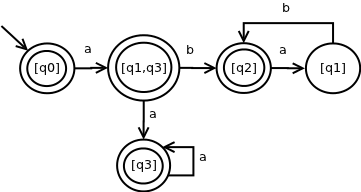
\includegraphics[scale=0.5]{dfa-from-nfa.png}
  \caption{DFA converted from NFA}
  \label{DFA}
\end{figure}

\end{enumerate}
\underline{\textbf{Pumping Lemma}}\\
\underline{E.g.}
Show that each of the following languages is not regular:
  \begin{enumerate}
  \item $\{a^i b^j | i > j\}$\\
  \\
  Proof by contradiction (using pumping lemma):\\
  Step 1: Assume $L$ is regular, then let $n$ be the constant in the lemma.\\
  \\
  Step 2: Select a specific string $z \in L$ such that $|z| \geq n$.\\
  $z = a^{n+1} b^n$\\
  \\
  Step 3: Split $z$ into $uvw$.\\
  By the lemma, $|uv| \leq n$, thus $v$ appears within the first $n$ characters
  ($v$ consists only of $a$'s).
  $z = uvw = a^q a^r a^s b^n$ where $u = a^q, v = a^r$, and $a^s b^n = w$.\\
  From the lemma we know:\\
  $q+r+s = n+1$\\
  $0 \leq |q| < n$\\
  $1 \leq |r| \leq n$ because $|v| \geq 1$\\
  $0 \leq |s|$\\
  $q+s < n + 1$\\
  \\
  Step 4: Find an $i$ such that $uv^iw \notin L$, violating the necessary condition.\\
  The lemma states that for $L$ to be regular, $uv^iw \in L$.\\
  If $i=0$, then $uv^0w = uw = a^q + a^s < n+1 \notin L$ (because there must be more $a$'s than $b$'s,
  and if one $a$ is missing, then it's false). Therefore $uw \notin L$ and $L$ is nonregular.  
  
  \item The set of strings over $\{0,1\}$ with an equal number of $0$'s and $1$'s.\\
  $L = \{w | w \in \{0,1\}^*$ and \# of $0$'s $=$ \# of $1$'s in $w\}$\\
  \\
  Intuition says we would need infinite states and thus a DFA would be impossible to build.
  Try pumping lemma.\\
  \\
  Select $z = 0^n 1^n \in L = uvw \in L$\\
  $|uv| \leq n$ so $v$ consists of $0$'s. $u = 0^q,\,v=0^r,\,w=0^s1^n$.\\
  We know $q+r+s = n$ and $n \geq |v| \geq 1$, so $q+s < n$.\\
  Lemma says $uv^iw \in L$ if regular. But for $i=0$, we have too few $0$'s in our string, since
  $uv^0w = uw = 0^q 0^s 1^n \notin L$ because $q+s < n$. Therefore $L$ is not regular.
  
  \item $\{a^i b^j c^{2j} | i \geq 0, j \geq 0\}$\\
  \\
  Select $z = a^n b^n c^{2n} \in L = uvw$.\\
  $|uv| \leq n$ so $v$ consists of $a$'s.\\
  $u = a^q, v = a^r, w = a^s b^n c^{2n}$.\\
  $q + r + s = n$\\
  Find an $i$ such $uv^iw \notin L$.\\
  $i = n+1 \rightarrow uv^{n+1}w = q + (n+1)r + s + n + 2n = q + r +s + n + 2n + nr = n + n + 2n + nr$\\
  Which is not in $L$ because then there would be more $a$'s than $c$'s. Thus $L$ is not regular.  
  
  \item The set of nonpalindromes over $\{a,b\}$.\\
  \\
  If $L$ is regular, then so is $\stackrel{-}{L}$ (the set of palindromes).\\
  $\stackrel{-}{L} = \{w\,|\,w \in \{a,b\}^*, w = w^R\}$. Use pumping lemma.\\
  Select $z = a^n b a^n = uvw$. $u = a^i, v=a^j, w=a^k b a^n$.\\
  $i+j+k=n$\\
  $i+k < n$\\
  $|uv| \leq n$\\
  $i + j \leq n$, so $n \geq j \geq 1$.\\
  Pump $v$ 0 times ($i=0$), we get $a^{i+k}b a^n \notin L$.\\
  Therefore $\stackrel{-}{L}$ is not regular and thus neither is $L$.
  \end{enumerate}
\underline{\textbf{Arbitrary}}\\
\textbf{Prove false:} Show a single example where it's false (proof by contradiction).\\
\\
\textbf{Cantor's Theorem:} For any set $A$, $|A| < |2^A|$\\
\\
\textbf{Sufficient \& Necessary Conditions:} $P \Rightarrow Q$: If $P$, then $Q$ ($P$ iff $Q$).
$P$ is a \underline{sufficient} condition for $Q$ to be true.
$Q$ is a \underline{necessary} condition for $P$ to be true.\\
$\bullet$ If $Q$ is false, we can say $P$ is false.\\
$\bullet$ If $Q$ is true, we cannot say anything about $P$.\\
\\
$\bullet$ $\emptyset$ is a language, but not a string\\
$\bullet$ $\epsilon$ is a not a language, but it is a string\\
$\bullet$ every language is infinite or has an infinite complement\\
$\bullet$ some languages are infinite and have an infinite complement
$L = \{w \in \{0,1\} \mid |w|$ is odd$\}$\\
$\bullet$ empty set $\emptyset$ is a subset of every language\\
$\bullet$ kleene closure of a language is not always infinite, $\emptyset$ and $\{\epsilon\}$\\
$\bullet$ concatenation of infinite language and finite language is not always infinite\\
\\
\underline{\textbf{Context-Free Grammar (CFG)}} \\
CFG's are used for describing the structure of programming languages and other artificial languages.
The idea is to use ``variables'' for sets of strings (i.e. languages). Variables are defined
recursively. Every production rule is of the form $V \rightarrow w$, where $V$ is a nonterminal
symbol (variable) and $w$ is a string on terminals and/or non-terminals (can be empty). \\
\\
\underline{E.g.}
Find CFG's for the following languages: \\
(start w/ base case \& use as many variables as needed)
\begin{eqnarray*}
  \{a^n b^n | n \geq 1\} & \{a^n b^n | n \geq 0\} \\
  S \rightarrow ab \,|\, aSb & S \rightarrow aSb \,|\, \epsilon \\
  \\
  (a+b)^*a & \{w | w \in (a+b) \mbox{ and } a's \neq b's\} \\
  S \rightarrow a \,|\, aS \,|\, bS & a = b,\, a > b,\, \mbox{ or } a < b \\
   & S \rightarrow U \,|\, V \\
  \mbox{Set of all production} & T \rightarrow aTbT \,|\, bTaT \,|\, \epsilon \\
  \mbox{rules for CFG's with} & U \rightarrow TaT \,|\, TaU \\
  T=\Sigma=\{a,b\}, \mbox{ and} & V \rightarrow TbT \,|\, TbV \\ 
  V=\{A,B,C\} &  \\
  S \rightarrow X \underline{\rightarrow} Y & \mbox{Set of strings over} \\
  X \rightarrow A \,|\, B \,|\, C & \Sigma = \{a,b,+,(,)\} \\
  Y \rightarrow \epsilon \,|\, aY \,|\, bY \,|\, AY \,|\, BY \,|\, CY & S \rightarrow a \,|\, b \,|\, S + S \,|\, (S)\\
  \\
  \{a^i b^j c^k | i \neq j \, or j \neq k\} & \{a^i b^j c^k | i,j,k > 0, i=j \mbox{ or } i=k\} \\
  i>j,\, j<i,\, j>k,\, \mbox{ or } j<k &  S \rightarrow XY \\
  S \rightarrow ABC \,|\, DEF \,|\, GHI \,|\, JKL & X \rightarrow aXb \,|\, ab \\
  A \rightarrow aA \,|\, a & Y \rightarrow cY \,|\, c \\
  B \rightarrow aBb \,|\, ab \,|\, \epsilon & \mbox{Similar for } i=k \\
  C \rightarrow cC \,|\, \epsilon & \\
  \mbox{Similar for } i<j, j>k, j<k & \{a^n w w^R a^n | n \geq 0, w \in \{a,b\}^* \} \\
  & \mbox{It's a palindrome} \\
  \mbox{Matching (nested) paranthesis} & S \rightarrow aSa \,|\, bSb \,|\, \epsilon \\
  S \rightarrow SS \,|\, (S) \,|\, () &
\end{eqnarray*}
\textbf{Parse trees} have the start symbol as the root, terminals as leaves, and variables as interior
nodes. Reading the leaves from left-to-right (preorder traversal) yields the derived string.\\
\\
A \textbf{derivation} of a string for a grammar is a sequence of grammar rule applications,
that transforms the start symbol into the string. A derivation proves that the
string belongs to the grammar's language. \\
In a \textbf{leftmost derivation}, the next nonterminal to rewrite is always the leftmost nonterminal;
in a \textbf{rightmost derivation}, it is always the rightmost nonterminal. \\
\\
\underline{E.g.} % Might have to reduce the size of this example!
Let $G$ be the grammar
\begin{eqnarray}
  S &\rightarrow& ASB \\
  S &\rightarrow& ab \\
  S &\rightarrow& SS \\
  A &\rightarrow& aA \\
  A &\rightarrow& \epsilon \\
  B &\rightarrow& bB \\
  B &\rightarrow& \epsilon
\end{eqnarray}

Leftmost derivation of string $aaabb$
  \begin{eqnarray}
    \setcounter{equation}{1}
    S &\Rightarrow& ASB \\
    \setcounter{equation}{4}
    S &\Rightarrow& aASB \\
    \setcounter{equation}{4}
    S &\Rightarrow& aaASB \\
    \setcounter{equation}{5}
    S &\Rightarrow& aa \epsilon SB = aaSB \\
    \setcounter{equation}{2}
    S &\Rightarrow& aaabB \\
    \setcounter{equation}{6}
    S &\Rightarrow& aaabbB \\
    \setcounter{equation}{7}
    S &\Rightarrow& aaabb\epsilon = aaabb
  \end{eqnarray}

  Rightmost derivation of the same string.
  \begin{align} % NOTE: eqnarray is discouraged (spacing issues), so trying align instead...
    \setcounter{equation}{0} % NOTE: setcounter works differently in align (-1)
    S &\Rightarrow ASB \\
    \setcounter{equation}{5}
    S &\Rightarrow ASbB \\
    S &\Rightarrow ASb \epsilon = ASb \\
    \setcounter{equation}{1}
    S &\Rightarrow Aabb \\
    \setcounter{equation}{3}
    S &\Rightarrow aAabb \\
    \setcounter{equation}{3}
    S &\Rightarrow aaAabb \\
    S &\Rightarrow aa \epsilon abb = aaabb
  \end{align}
A context-free grammar is said to be \textbf{ambiguous} if there exists a string that can be
generated by the grammar in more than one way (i.e. the string admits more than one parse tree or,
equivalently, more than one leftmost derivation).
$\{a^i b^j c^k | i=j \mbox{ or } i=k\}$ is \emph{inherently ambiguous.} \\
\\
\underline{E.g.} % TODO: Might have to reduce the size of this example!
  Give an unambiguous grammar equivalent to $G$. \\
  \\
  Some ambiguous grammars can be converted into unambiguous grammars, but no general procedure
  for doing this is possible just as no algorithm exists for detecting ambiguous grammars.
  So instead we describe what type of strings $G$ produces and then try to find a grammar that
  (1) is equivalent to $G$ (i.e. generates the same language), and (2) is unambiguous
  (i.e. for every sentence of the language, the parse tree is correct).\\
  \\
  $G$ produces strings that start with an $a$ and end with a $b$ and have any combination of $a$'s and
  $b$'s in between.
  \begin{align*}
    S &\Rightarrow aTb \\
    T &\Rightarrow aT \,|\, bT \,|\, \epsilon
  \end{align*}
\textbf{Useless Symbols}\\
Sometimes $S$ derives nothing which means the language is empty.
This is the case when you cannot reach a terminal string.
To reach a terminal string you need a production of the form $A \rightarrow w$. \\
To eliminate useless symbols (1) Eliminate symbols that derive no terminal string,
(2) Eliminate unreachable symbols. \\
\\
\underline{\textbf{Context-Free Language (CFL)}} \\
CFL is a language generated by a CFG.
If CFL, give a PDA or CFG. If not CFL, show with pumping lemma. \\
\\
\underline{E.g.}
Show that the following languages over $\Sigma = \{a,b\}$ are not CFL (using pumping lemma).
NOTE: Have to prove for \emph{every} case it can violate (not done here).
\begin{enumerate}
  \item % a
  The set of strings of $a$'s, $b$'s, and $c$'s, with an equal number of each. \\
  \\
  Intuition tells us it is not CFL because you would need to count, which we cannot do.
  So we should with pumping lemma that it is not CFL.
  There are many cases where it will violate the language property, we just need one.
  \begin{align*}
    \mbox{Let } z &= a^n b^n c^n \\
    &= u v^i w x^i y \\
    |vwx| \leq n \\
    |vx| \geq 1 \\
    v,x \mbox{ contains } a's: \\
    \overbrace{\underbrace{a \cdots a}_{uvwxy}}^{n} \overbrace{b \cdots b}^{n} \overbrace{c \cdots c}^{n} \\
    u v^i w x^i y \notin L \mbox{ if } i \geq 2
  \end{align*}

  \item % b
  $\{ww^Rw|w \in \Sigma^*\}$ \\
  \\
  Intuition tells us it is not CFL, because we would need more than one stack to match.
  So we try disproving with pumping lemma.
  \begin{align*}
    \mbox{Let } z &= a^n a^n a^n \\
    &= u v^i w x^i y \\
    |vwx| \leq n \\
    |vx| \geq 1 \\
    v,x \mbox{ contains } a's: \\
    \overbrace{\underbrace{a \cdots a}_{uvwxy}}^{n} \overbrace{a \cdots a}^{n} \overbrace{a \cdots a}^{n} \\
    u v^i w x^i y \notin L \mbox{ if } i \geq 2
  \end{align*}
  \item % d
  $\{a^p|p$ is a prime$\}$ \\
  \\
  Intuition says it is not CFL because we would need to calculate primes.
  If $|\Sigma| = 1$, then both versions of the pumping lemma (CFL and regular languages)
  become the same, and we already proved it in class for the regular language example.
  So we can safely say that this is not CFL.
\end{enumerate}
Grammar $G = (V, \Sigma, P, S)$ \\
type 0 (unrestricted): $\alpha \rightarrow \beta$ (e.g. $aAa \rightarrow aa$) \\
type 1 (context-sensitive): $\alpha \rightarrow \beta$ and $|\alpha| \leq |\beta|$ iff $\beta \neq \epsilon$ \\
type 2 (context-free): $\alpha$ is a single variable (e.g. $A \rightarrow ...$) \\
type 3 (regular grammar): $A \rightarrow aB \,|\, a \,|\, \epsilon$ \\
\\
\underline{\textbf{Push Down Automata (PDA)}} \\
A PDA is a stack with operations push \& pop. It models a parser.
In language-defining power, it's equivalent to a CFG.
You can only have a single stack, which limits the power of PDA.
The moves for a PDA are determined by (1) the current state, (2) the current input symbol, and
(3) the current symbol at the top of the stack.
PDA's are non-deterministic, so it can have a choice of next moves.
In each choice, the PDA can (1) change state, and (2) change the top stack symbol. \\
\begin{tabular}{c l}
 & $M = \{Q, \Sigma, \Gamma, \delta, q_0, Z_0, F\}$ \\
$Q:$ & finite set of states \\
$\Sigma:$ & input alphabet \\
$\Upgamma:$ & stack alphabet \\
$\delta:$ & transition function \\
$q_0:$ & start state ($q_0 \in Q$) \\
$Z_0:$ & start symbol ($Z_0 \in \Upgamma$) \\
$F:$ & set of final states ($F \subseteq Q$)
\end{tabular}
\\ \\
\underline{E.g.}
Construct PDA for the following languages and state if
``accept by empty stack'' or ``accept by final state.'' \\
\textbf{TIP:} draw out a sample string and corresponding stack.

\begin{enumerate}
  \item % a
  $\{w|w \in (a+b)^+$ and contains the same number of $a$'s and $b$'s$\}$  \\
  \\
  We match the $a$'s and $b$'s by pushing and popping.
  If the stack ever becomes empty, we have the same numbers of $a$'s and $b$'s.
  We will accept this language by empty stack, so the stack will start out with empty stack
  symbol $Z_0$ and finish with no symbols.
  \\
  \begin{align*}
    \delta(q_0, a, Z_0) &= \{(q_0, AZ_0)\} \mbox{ push A on empty stack} \\
    \delta(q_0, b, Z_0) &= \{(q_0, BZ_0)\} \mbox{ push B on empty stack} \\
    \delta(q_0, a, A) &= \{(q_0, AA)\} \mbox{ keep pushing A} \\
    \delta(q_0, b, B) &= \{(q_0, BB)\} \mbox{ keep pushing B} \\
    \delta(q_0, a, B) &= \{(q_0, \epsilon)\} \mbox{ `a' encountered, pop B} \\
    \delta(q_0, b, A) &= \{(q_0, \epsilon)\} \mbox{ `b' encountered, pop A} \\
    \delta(q_0, \epsilon, Z_0) &= \{(q_0, \epsilon)\} \mbox{ end of input, pop } Z_0
  \end{align*}
  
  \item % b
  $\{ww^R|w \in (a+b)^+\}$ \\
  \\
  This PDA will recognize the language of even length palindromes (with length greater than 0)
  over $\Sigma = \{a,b\}$. This PDA pushes the input symbols on the stack until it guesses that it is
  in the middle and then it compares the input with what is on the stack, popping off symbols from the
  stack as it goes. If it reaches the end of the input precisely at the time when the stack is empty,
  it accepts. Thus it accepts by empty stack, and it is non-deterministic.
  We need two states ($q_0$ for pushing, $q_1$ for popping) because we need the same number of
  $a$'s and $b$'s (like in the previous language), \emph{and} it must be a palindrome.
  \begin{align*}
    \delta(q_0, a, Z_0) &= \{(q_0, AZ_0)\} \mbox{ push A} \\
    \delta(q_0, b, Z_0) &= \{(q_0, BZ_0)\} \mbox{ push B} \\
    \delta(q_0, a, A) &= \{(q_0, AA), (q_1, \epsilon)\} \mbox{ push or pop A} \\
    \delta(q_0, b, B) &= \{(q_0, BB), (q_1, \epsilon)\} \mbox{ push or pop B} \\
    \delta(q_0, a, B) &= \{(q_0, AB), (q_1, \epsilon)\} \mbox{ push or pop A} \\
    \delta(q_0, b, A) &= \{(q_0, BA), (q_1, \epsilon)\} \mbox{ push or pop B} \\
    \delta(q_1, a, A) &= \{(q_1, \epsilon)\} \mbox{ pop A} \\
    \delta(q_1, b, B) &= \{(q_1, \epsilon)\} \mbox{ pop B} \\
    \delta(q_1, a, B) &= \{(q_1, \epsilon)\} \mbox{ pop A} \\
    \delta(q_1, b, A) &= \{(q_1, \epsilon)\} \mbox{ pop B} \\
    \delta(q_1, \epsilon, Z_0) &= \{(q_1, \epsilon)\} \mbox{ end of input, pop } Z_0
  \end{align*}
\end{enumerate}
\underline{\textbf{Turing Machine (TM)}} \\
\# of TM is infinitely countable, \# of languages is infinitely uncountable,
so there are language that have no TM (i.e. uncountable unsolvable problems).

\emph{TODO: Creating a TM and formal definitions}
\\
\underline{\textbf{Undecidable Problems}} \\
\underline{E.g.} Let $ALL_{CFG} = \{<G> |\, G$ is a CFG and $L(G) = \Sigma^*\}$.
It is known that this language is undecidable.
Define $EQ_{CFG} = \{<G,H> |\, G$ and $H$ are CFG's and $L(G) = L(H)\}$.
Show that $EQ_{CFG}$ is undecidable. \\
\\
Use reduction. Show we can solve $ALL_{CFG}$, then we can solve $EQ_{CFG}$.
But $ALL_{CFG}$ is known to be unsolvable, so then $EQ_{CFG}$ is also unsolvable since
$ALL_{CFG} \leq EQ_{CFG}$. $ALL_{CFG}$ reduces to $EQ_{CFG}$, so $EQ_{CFG}$ is at least as hard
as $ALL_{CFG}$. \\
\\
\underline{E.g.} Given $A = \{<M> |\, M$ is a finite automaton and $L(M) = \Phi\}$
where $M$ is some encoding of the machine $M$. Is $A$ Turing-decidable? \\
\\
A FSM of $n$ states accepts strings of length $< n$, so brute force!
Generate all strings of length $< n$, see if any is accepted. Guaranteed to halt (Turing-decidable).\\

\emph{TODO: Formal proofs}
\\
\underline{\textbf{Chomsky Hierarchy of Languages}} \\
\begin{tabular}{c l}
Regular: & $\cdot$ regular expression \\
& $\cdot$ FSM (DFA, NFA, NFA w/ $\epsilon$-moves) \\
& $\cdot$ closure properties \\
Not Regular: & $\cdot$ pumping lemma ($uv^iw$)\\
& $\cdot$ DFA w/ infinite states \\
& $\cdot$ intuition says calculate or inf. memory \\
\hline
CFL: & $\cdot$ PDA (e.g. palindromes) \\
& $\cdot$ CFG (easier) \\
Not CFL: & $\cdot$ pumping lemma ($uv^iwx^iy$) \\
\hline
Recursive: & $\cdot$ decidable (algorithm/TM always terminates) \\
Rec. Enumerable: & $\cdot$ recognizable (terminates iff legal input) \\
Non-Rec. Enum.: & $\cdot$ unsolvable (doesn't fit elsewhere) \\
\hline
\end{tabular}
Recursively Enumerable languages are closed under:
\begin{enumerate}
  \item Kleene closure ($L^*$ of $L$)
  \item concatenation ($L \cdot P$)
  \item union ($L \cup P$)
  \item intersection ($L \cap P$)
\end{enumerate}
They are \underline{not} closed (i.e. not guaranteed to be RE) under:
\begin{enumerate}
  \item set difference ($L - P$)
  \item complementation ($\bar{L}$ of $L$)
\end{enumerate}
\begin{tabular}{l | c}
$L_1 = \{a^i b^j c^k | i,j,k > 0, i=j$ or $i=k\}$ & CFL \\
$L_2 = \{a^i b^j c^k | i = k, j > 2\}$ & CFL \\
$L_3 = \{0^n | n$ is multiple of $101\}$ & REG \\
$L_4 = \{0^i 1^j 2^k | i + j = k\}$ & CFL \\
$L_5 = \{<M,w> | w \in \Sigma^*, M = DFA, M$ accepts $w\}$ & REC \\
$L_6 = \Sigma$ & REG \\
$L_7 = A_{TM}$ Halting Problem & R.E. \\
$L_8 =$ finite set & REG \\
$L_9 =$ union of any finite \# of R.E. languages & R.E. \\
$L_{10} = \{wxw^R | w,x \in (0+1)^+\}$ & REG \\
$L_{11} = \{\} = \emptyset = $ empty language & REG \\
$L_{12} = \{a^{p+1} | p$ is prime$\}$ & REC \\
$L_{13} = \{xy | x \in L$ and $y \notin \Sigma^* - L\}$, L is regular & REG \\
$L_{14} =$ intersection of any finite \# of R.E. languages & R.E. \\
$L_{15} = \{a^i b^j | i,j > 0\}$ & REG \\
$L_{16} = \{w | w \in \{a,b\}^*, w$ is a palindrome$ \}$ & CFL \\
$L_{17} = \{<M> | M$ is a TM, M does not accept $<M>\}$ & N.R.E. \\
$L_{18} = L(G), G: S \rightarrow Sa | Sb = \emptyset$ (no terminal string)  & REG \\
$L_{19} = \{w | w \{a,b\}^*$ and \# $ a's = $\# $ b's \}$ & CFL \\
$L_{20} = \{a^i b^j a^k | i = j = k\}$ & REC \\
\end{tabular}
\begin{figure}[h!]
  \centering
    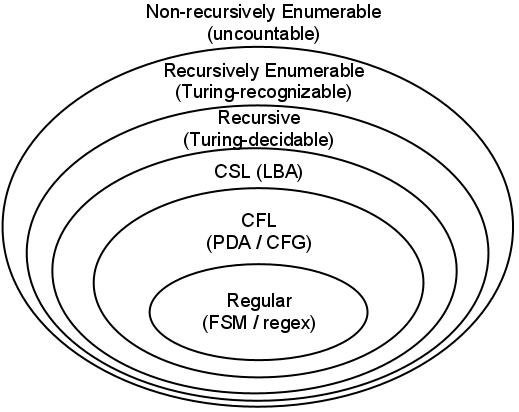
\includegraphics[scale=0.5]{ChomskyHierarchy.png}
  \label{CH}
\end{figure}
\end{document}